% ****** rbf.tex ******
% Este archivo provee el formato para la Revista Boliviana de Fisica, RBF.
\documentclass{rbf}
%\documentclass[onecolumn]{rbf}

\usepackage{amsmath}
\usepackage{natbib}
\usepackage[utf8]{inputenc}
%\usepackage[latin1]{inputenc}

%%%%%%%%%%%%%%%%%%%%%%%%%%%%%%%%%%%%
\newcommand{\mr}{{\bf RBF: }}
\newcommand{\jim}{{\bf JY: }}

\begin{document}

\title{El caos y su trascendencia: entrevista con James Yorke \\Chaos and its transcendence: interview with James Yorke}

\author{Gonzalo Marcelo Ramírez-Ávila\marca{*}}
\afil{Instituto de Investigaciones Físicas, Universidad Mayor de San Andrés, Campus Universitario c. 27 Cota-Cota, Casilla 8635, La Paz, Bolivia
}%

\alpie{*}{http://www.fiumsa.edu.bo/docentes/mramirez/}% Las lineas se cortan automaticamente o puede obligarse esto con

\begin{abstract}
\Resumen
James Yorke es uno de los científicos más prominentes e influyentes en lo que concierne a la teoría del caos pues fue el acuñador de este término en la jerga científica. En octubre de 2016 coincidí con este personaje en Dresde, Alemania, donde consideré que sería importante hacerle una entrevista para la Revista Boliviana de Física con el fin de motivar a la comunidad de físicos bolivianos en el estudio de la dinámica no lineal.
\descriptores{Biografías, tributos, notas personales -- Control del caos, aplicaciones del caos}

Código(s) PACS: 01.60.+q, 05.45.Gg

\Abstract
James Yorke is one of the most prominent and influential scientists in which concerns chaos theory since he was the one who proposed this term in scientific jargon. In October 2016 I met this personage in Dresden, Germany, where I thought it would be appropriate to do an interview for the Bolivian Journal of Physics to motivate the community of Bolivian physicists in the study of nonlinear dynamics.
\keywords{Biographies, tributes, personal notes -- Control of chaos, applications of chaos}
\end{abstract}

\maketitle

%%%%%%%%%%%%%%%%%%%%%%%%%%%
%   INTRODUCCION
%%%%%%%%%%%%%%%%%%%%%%%%%%%

\section{Introducción}\label{intro}
Corrían los primeros días del mes de octubre de 2016 y en el Instituto Max Planck para la Física de los Sistemas Complejos (MPIPKS, por su sigla en alemán) en Dresde, Alemania, tiene lugar el taller ``Multistability and Tipping: From Mathematics and Physics to Climate and Brain". Entre los conferencistas invitados estaba James A. (Jim) Yorke (JY). Durante los días del evento, observé que JY seguía con  atención muchas de las charlas y participaba activamente formulando preguntas muy inteligentes que permitían que los expositores lograsen aclarar los puntos más importantes de sus temas. El último día del evento, le propuse hacerle una entrevista para la Revista Boliviana de Física (RBF) y muy gentilmente, a pesar de que varios otros participantes lo requerían para diferentes aspectos, me concedió parte de su valioso tiempo, en el que no solo hicimos la entrevista sino también me hizo una demostración experimental del comportamiento caótico de un péndulo doble y también recibí de su parte algunos consejos que podrían ayudar a mejorar mi actividad científica.

Antes de presentar la transcripción de la entrevista, es bueno hacer un breve resumen de la vida y obra de JY (ver Fig.~\ref{JY}) con información obtenida de \cite{WIKI17}. Obtuvo su doctorado en la Universidad de Maryland en 1966 y posteriormente trabajó en esa institución hasta llegar a ocupar el puesto de profesor y detentar una cátedra en el Departamento de Matemática de donde se jubiló oficialmente en junio de 2013, aunque sigue muy activo en sus actividades científicas. Tuvo una prolífica labor tanto académica como científica, habiendo dirigido más de 50 tesis doctorales y tener más de 600 publicaciones como se ve en \cite{GS17}, entre las cuales se destacan por su impacto, el control del caos planteado por \cite{OTT90} y que hasta les valió una nominación al premio Nobel en 2016; el trabajo donde por primera vez se introduce el término ``caos" expuesto por \cite{LI75} y que tiene una gran importancia desde el punto de vista histórico como lo establecieron \cite{AUBIN02}; y el método de reconstrucción de espacios de fases a partir de series temporales desarrollados por \cite{SAUER91}, el mismo que sirvió como base de una investigación del Grupo de Sistemas Complejos de la UMSA, llevada a cabo por \cite{GERARD16}, donde se caracterizaron los sonidos de tarkas utilizando estas técnicas.
\begin{figure}[htbp!]
 \centering
  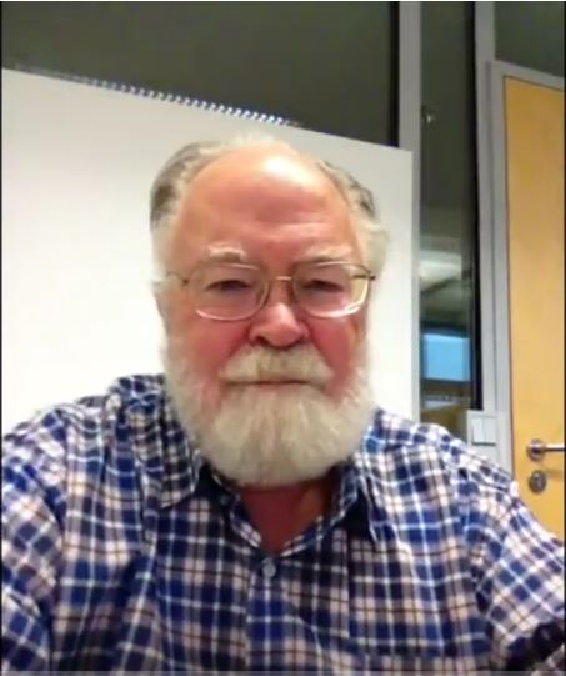
\includegraphics[width=0.4\textwidth]{Jim_Yorke.pdf}
 \caption{James A. Yorke (nacido el 3 de agosto de 1941 en Plainnfield, Nueva Jersey, EEUU). Es un Investigador Distinguido y Profesor de Matemática y Física y además de ex Director del Departamento de Matemática de la Universidad de Maryland en College Park, como se menciona en \cite{WIKI17}. Foto tomada en Dresde el sábado 8 de octubre de 2016 en el MPIPKS.}
 \label{JY}
\end{figure}

\section{Entrevista}\label{inter}
\mr Estamos con Jim Yorke quien es quizás uno de los científicos más conocidos, en el campo de la dinámica no lineal y quisiera preguntarle ¿Cuál fue su principal motivación para estudiar la no linealidad?

\jim Bueno, antes de empezar en dinámica no lineal, yo estaba estudiando ciertas áreas de geometría diferencial. Luego, cuando me interesé en la dinámica simplemente visualicé el movimiento, cómo se mueven la cosas generando cambios y pensar en la idea del cambio como un todo, es simplemente un área perfecta en la cual trabajar. Realmente me gustó, estaba encantado puesto que podía relacionarme con eso. A veces sistemas con retardos temporales, o derivadas múltiples, dan una muy buena noción del cambio.

\mr El periodo 3 implica caos, ¿Qué representa esto para usted? y ¿cuál es el origen y la razón para haber elegido la palabra ``caos"?

\jim Para mí, todos saben lo que es el caos puesto que la vida de todos es caótica. El caos significa que un pequeño cambio en un momento crucial, puede provocar un enorme cambio en tu vida; lo mismo sucede con ciertos circuitos eléctricos y una gran variedad de cosas. El caos significa que pequeños cambios producen grandes cambios. Han habido películas acerca del caos donde, por ejemplo, el cierre repentino de una puerta del tren subterráneo que evita el ingreso en este de una mujer que corría, y luego te muestran como evoluciona su vida. Después, repiten parte de la escena pero esta vez, ella logra entrar al vagón, lo que produce un cambio radical en la evolución de su vida. Existe otra película acerca del caos, llamada ``La Avispa'', una pequeña película donde se muestra a una persona conduciendo su auto y una avispa zumbando sobre su cabeza; el conductor coge y agita un periódico con el fin de matar a la avispa pero falla en su intento, lo que provoca que la avispa le pique trayendo como consecuencia el choque de su auto. Este hecho, se constituye en el inicio de una espiral descendente en su vida. Al igual que en la anterior película, se repite la escena pero ahora el conductor acierta y mata a la avispa y su vida transcurre normalmente y todo está bien. Dependiendo si matas a la avispa o no,
tu vida podría transcurrir de manera muy diferente, ..., de eso se trata el caos. Usualmente vemos aspectos matemáticos, en los cuales, pequeños cambios producen grandes cambios.

\mr El control de caos, un trabajo muy importante ¿Cuáles son los principales aspectos y consecuencias del mismo?

\jim Debo decir que este es uno de nuestros trabajos que tuvo un gran impacto, pero lo tuvo por una extraña razón, siendo esta, el hecho de que los físicos generalmente no aprenden acerca de teoría de control\footnote{Actualmente en la Carrera de Física de la UMSA, se tiene una materia denominada ``Teoría de Control" a cargo del Ing. Pedro Miranda.}; en cambio, los ingenieros normalmente aprenden de teoría de control; en tanto que los matemáticos lo hacen a veces, pero los físicos nunca. Entonces, cuando empezamos a decirles como podrían usar en sus experimentos el control del caos, haciendo, por ejemplo, un pequeño cambio en la resistencia eléctrica o un pequeño cambio en la corriente y podrían determinar que ocurrirá en sus sistemas caóticos. Les gustó mucho y pensaron que era una gran idea; entonces, lo que hicimos fue explicarles a los físicos acerca de la teoría de control y lo que también hicimos fue decirles cómo podrían controlar sus experimentos sin tener un modelo matemático de los mismos. Porque después de todo, es difícil tener un modelo exacto de un experimento. Consiguientemente, les comentamos
que simplemente podían ver el sistema dinámico y cómo este evoluciona y que podrían crear un conjunto de datos para el cual encontraran órbitas periódicas que con pequeños cambios en, digamos, la resistencia de un circuito, podrían ver la dinámica de la órbita que es casi periódica y ajustando la resistencia hacia atrás y adelante a manera de retroalimentación, podrían controlar el circuito y podrían mantenerlo periódico a pesar de que este sería intrínsecamente caótico si se mantuviese la resistencia constante. Se podría también ajustar ligeramente la resistencia y provocar una migración a una órbita periódica diferente y conseguir estabilizaría. Todo lo anterior, sin tener ecuación alguna. De eso se trata el control del caos.

\mr En su opinión, ¿cuál es el estado del arte en la teoría del caos?

\jim Sorprender es una naturaleza del caos, sorprender a la gente. Nunca sé en qué dirección avanzo. Esperaría hacer descubrimientos que me sorprendan y por ende, no puedo planear cómo sorprenderme. Así, hablo con la gente, ellos toman ideas, yo obtengo ideas, trabajamos juntos y nos sorprendemos a nosotros mismos
y el caos nos sorprende. Entonces, la dirección a la cual se dirige el caos es difícil de decir pero hay una tendencia a que sea encaminado hacia aplicaciones. A pesar de ello, yo sigo interesado en estudiar los fundamentos de la teoría del caos. Nuevamente, no sé a dónde nos llevará esto. Una forma de ver esto, es realizar experimentos numéricos; tengo un programa: ``Dynamics" que escribí, el cual se encuentra disponible en mi página web\footnote{Un libro de utilización de este software fue escrito por \cite{NUSSE94}}. Lo utilizo para explorar sistemas y encontrar cosas nuevas que prácticamente no esperaba; eso es muy interesante para mí. Está claro que al ver ejemplos y constatar que son sorprendentes, se debe tener experiencia en caos.

\mr ¿Cuáles considera que son los desafíos principales para la dinámica no lineal?

\jim Los desafíos para sorprender. Me gusta la investigación, no sólo los detalles de cómo función algo en particular, sino encontrar cosas que la gente no esperaría que estén ahí. Por ejemplo, encontramos y fuimos unos de los primeros en publicar acerca de fronteras de las cuencas, cuencas de atracción para sistemas físicos y encontramos que en el estudio de sistemas matemáticos muy abstractos y de variable compleja que se aplicaban a sistemas físicos en muchas maneras. Luego descubrimos ``cuencas acribilladas", las cuales son mucho más raras que la cuencas regulares de atracción; son tan raras que la gente no esperaba que existan y de repente, ... ahí están y ocurren en muchos casos. Controlar el caos es algo que no se esperaba pero de repente empezamos a pensarlo; reflexionamos acerca de los límites de lo que es conocido y así buscar sistemas que son ligeramente diferentes; por ejemplo, sistemas continuos que tienen derivadas discontinuas
y qué tipos de bifurcaciones experimenta el sistema; exploramos ese tipo de sistemas, ... estamos permanentemente explorando.

\mr Algunas personas dicen que la ciencia no lineal es la ciencia del siglo XXI ¿Cómo considera está afirmación?

\jim Yo diría que la dinámica no lineal es la ``ciencia del todo" porque un sistema debería ser horriblemente especial para ser lineal. La Mecánica Cuántica se comporta de manera diferente pero eso es porque se lidia con ondas de probabilidad pero si uno se fija en un sistema caótico y ve la distribuciones de probabilidad y cómo evolucionan estas en el tiempo, se comportan casi como lo hacen las funciones de onda pero como en casi todos los sistemas, pequeños cambios resultarán en grandes cambios. Una vez, quise preguntar a una joven mujer
que estaba asistiendo a una clase, cómo se conocieron sus padres. Esto fue en Wisconsin, ella dijo que su madre tomó un taxi y empezó a hablarle al conductor, congeniaron, quedaron para volverse a ver y finalmente se casaron. Esta muchacha fue el resultado de esto. Entonces, ¿dónde estuviese esta joven si su madre hubiese tomado otro taxi? De eso trata el hecho de que pequeños cambios van produciendo grandes cambios; no sólo un evento, sino eventos una y otra vez. A veces los estudiantes postulan a una universidad en la que no son aceptados y creen que su vida está destruida por esto; pero luego van a otra universidad donde la pasan muy bien y es perfecta para ellos. Lo que la teoría del caos nos dice es que a pesar de que debemos planear el futuro, también debemos estar preparados para cambiar nuestros planes. La gente más exitosa es aquella que es buena en el plan B.

\mr Acerca de esto, ¿considera que estas propiedades características del caos están en cierta forma relacionadas con el concepto de serendipia?

\jim La serendipia tiene que ver con el plan B. Se tiene originalmente un plan A y de pronto aparece una oportunidad y uno toma esta oportunidad. La serendipia significa que uno toma la oportunidad y algo nuevo aparece. La persona que creo Amazon llamado Jeffrey Bezos señala que la mayoría de los arrepentimientos no son por haber hecho algo, sino por no haberlo hecho; los arrepentimientos son por omisión
más que por comisión.

\mr En lo que concierne a premios, de los que usted obtuvo importantes galardones, ¿Cuál es su opinión, por ejemplo, respecto a la medalla Fields?

\jim La medalla Fields identifica a personas extremadamente brillantes y en cierta forma es mejor que el premio Nobel en el sentido de que las personas en matemática, una vez cumplidos los 40, saben que no deben preocuparse sin importar lo inteligentes que sean. Así, pueden dejar de preocuparse por esto; en cambio, se ve a físicos preocupados por obtener el premio Nobel y de manera realista, en la mayoría de los casos, hay mucha gente que está muy cerca de ganar el premio Nobel o que lo merecen. Ahora mismo tienen el problema del experimento LIGO acerca de la gravedad y a quién darle el premio Nobel. Hay muchas situaciones en las cuales te preguntas en cómo te sentirías si
estuvieses trabajando en un determinado campo y les dieran el premio Nobel a tres de tus colaboradores y considerases que tú fuiste el cuarto colaborador y no pueden dártelo pues sólo se lo otorga como máximo a tres personas y que por esa razón te dejaron fuera... tendrías un sentimiento terrible. Los medallistas Fields no tienen que preocupar por esto puesto que no se comparte el premio con colaboradores sino solo se otorga la medalla a gente brillante y cuando se llega a los 40 ya no es motivo de preocupación\footnote{En 2003, JY compartió la importante distinción ``Japan Prize" con Bénoit Mandelbrot por sus trabajos en caos y fractales respectivamente. Este premio está dotado de una suma de 50 Myenes que en dólares americanos representa aproximadamente la suma de 458 300. Detalles del premio otorgado a JY, los da \cite{SANJUAN03}.}.

\mr Vamos a pasar ahora a algunas aspectos relacionadas con Bolivia y la física en general. Hablando de la especialización de un Departamento de Física, ¿por qué considera que el mismo debiese estar bastante especializado? y ¿cuál debiera ser el criterio para escoger las áreas principales en uno que estuviese en Bolivia?

\jim A medida que la ciencia evoluciona, habrá en cierta forma más especialización; por lo que si hace 15 años se tenían grupos especializados en relatividad general, ahora se tienen grupos especializados en el experimento LIGO que es un subconjunto de la temática gravitacional. Pienso que una universidad como la de La Paz debiera hacer, es intentar ser la mejor universidad para que pueda formar y atraer a la mejor gente posible. Lo anterior no implica cubrir todas las áreas de la física; hay muchas universidades en Latinoamérica y un estudiante tal vez no pueda ir a una universidad específica, y mas bien, debiera escoger una universidad donde en lo posible haya un centro de excelencia. Por supuesto que puede ser difícil ir a otro país pero aún así, lo que atrae es la excelencia. Opino que la universidad debiera preguntarse: ``¿en qué áreas puede ser fuerte y sobresalir?" y cada año, cuando contrate nuevo personal académico y de investigación, debiera cuestionarse ``¿quién es la mejor persona que se pueda contratar?" Esa persona usualmente será alguien estrechamente relacionado a uno de los grupos y no significa un ex-estudiante de uno de los grupos sino un buen investigador que tenga una visión independiente pero que pueda colaborar con la gente de dicho grupo. se construye la mejor universidad teniendo a un personal que coadyuve en las principales tareas del Departamento. En general, los ex-estudiantes son las personas más interesadas en esto y los que más compenetrados están en los aspectos de enseñanza y trabajo con los estudiantes, lo que es un aspecto primordial puesto que sin eso, no tendría mucho sentido el tener una universidad ¿verdad? Lo más importante son los estudiantes.

\mr ¿Cuáles son las formas de motivar en la gente joven el estudio de la Física en general y el de la dinámica no lineal en particular?

\jim Cuando yo estaba en colegio, podíamos ir a la tienda de la esquina y comprar libros de bolsillo acerca de ciencia, cosas que podían ser leídas por el público en general. Yo hice eso; por ejemplo, habían libros acerca de relatividad y cosmología y de muchos otros temas como ser la biología. Con esa experiencia, me enfoqué en la importancia de ofrecer libros que no sean caros para el público. Tengo un libro acerca de dinámica no lineal, y escogimos la editorial Springer que nos da los precios más baratos para el público, lo cual fue nuestro criterio. Ellos han mantenido el precio bastante razonable y tienen ediciones especiales para muchos países, probablemente también para Bolivia. Cuando se escribe un libro, no se gana mucho dinero, por lo que pensar en cuánto dinero se ganará es irrelevante. Se trata mas bien de a quiénes se va a influenciar, a quiénes se pueden inspirar. También hay revistas
científicas de divulgación como ``science news'' que leí desde que estaba en colegio. Esta revista bi-semanal viene con artículos de todas las ciencias; algunos de ellos son interesantes y otros no. De todos modos, un estudiante debería tratar de averiguar tanto como pueda de todo tipo de áreas: física, astronomía, biología, matemática, ... Conocer áreas, no leyendo textos muy complicados sino leyendo cosas fácilmente accesibles para estudiantes.

\mr En referencia a publicaciones, ¿considera que es importante mantener la RBF a pesar de todas las dificultades en relación a la edición  de esta?

\jim No sé nada acerca de la RBF.

\mr Le puedo informar que es una revista que tiene unos 20 años de antigüedad y el principal objetivo de esta es publicar las investigaciones desarrolladas por personas de los diferentes Departamentos de Física en Bolivia. Al principio funcionó muy bien pero ahora hay un leve declive porque la gente que puede publicar prefiere hacerlo en una revista internacional. Por ello, la RBF se encuentra en una situación de carencia de artículos actualmente.

\jim Creo que algo interesante de hacer sería diseñar sitios web puesto que se constituyen en un recurso. Es un poco diferente pues por ejemplo, si se quisiese saber ¿qué tipo de artículos están publicando los investigadores de los departamentos de Física en Bolivia? entonces, se podría tener una lista de dichos artículos y quizás dónde se encuentran. Muchas veces, estos artículos están disponibles de manera gratuita en arXiv. También podrían tener en el sitio web artículos científicos interesantes para audiencias generales como que haya un artículo acerca de LIGO, explicando de qué se trata y qué se está intentando hacer; o que haya un artículo sobre CRISPR\footnote{Herramienta de edición genómica.} que es un tema de biología en el cual se tiene un tremendo avance puesto que mediante esta herramienta, se puede insertar genes; o artículos de divulgación de inteligencia artificial en los cuales, la palabra ``profundo'' aparece una y otra vez, como ``pensamiento profundo" y ``azul profundo"\footnote{Computadora jugadora de ajedrez que enfrentó y derrotó en 1997 al entonces campeón mundial de ajedrez Garry Kasparov tal como se señala en \cite{WIKI97}.}; significa que tienen inteligencia artificial, siendo conjuntos de redes interactuantes de muchas capas. Las denominadas redes complejas de multicapas o redes de redes se están volviendo tremendamente importantes. En realidad, este concepto cobró importancia en los últimos cinco años. Entonces, ¿dónde están los artículos de divulgación que un estudiante de colegio pueda leer? Quizás podría haber un recurso que los lleve a dichos artículos
sin tener el artículo en el sitio web. Se podría preguntar a los visitantes del sitio:  ¿cuál es su artículo favorito?, ¿cuál es el mejor artículo que leyó en el último año? Eso serían para las personas más técnicas. También, comentar libros interesantes como ser alguno que trate de cómo evolucionó la vida y cómo las células complejas evolucionaron de bacterias, habiendo dos tipos de bacterias y a las que se bacterias y arqueas, que en cierta forma se unieron y una se convirtió en una celda de potencia para la otra. Así de repente, la célula tendría una celda de potencia independiente y podía tener muchas copias de estas. Lo anterior marcó la diferencia, pero estas células complicadas también evolucionaron en muchas estructuras que tenían núcleo, cosa que las bacterias no tenían. Así, estas células tenían  celdas de potencia, sexo, motilidad, paredes flexibles, etc. Todas estas cosas ocurren en casi todas las células complejas y no así en las bacterias. Entonces, es un libro fascinante. También es bueno para los físicos porque explica cómo la energía potencia a las células; ese es el tema central.

\mr Para terminar esta entrevista, ¿podría dar un mensaje a la comunidad de físicos de Bolivia?

\jim Mi mensaje a los futuros físicos y a los actuales es que no piensen con demasiada anticipación, no intenten planear toda su vida
no digan: ``Voy a escribir 4 artículos acerca de algún tema'', sólo exploren el tema y encuentren las cosas más sorprendentes que puedan
y estén listos para cambiar al plan B cuando se presente una oportunidad.

Al finalizar la entrevista, JY quiso hacer una demostración experimental del caos, utilizando para ello, un péndulo doble que se muestra en la Fig.~\ref{JY2} y cuyo vídeo está disponible en \cite{YT16}.
\begin{figure}[tbp!]
 \centering
  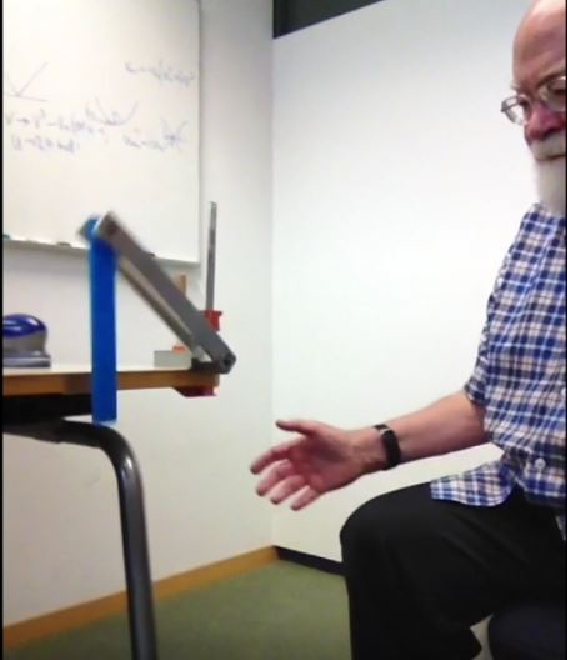
\includegraphics[width=0.4\textwidth]{Jim_Yorke_2.pdf}
 \caption{Péndulo doble en funcionamiento y que presenta una gran variedad de comportamientos, desde regulares hasta caóticos. El vídeo mostrando el movimiento de este péndulo en diferentes situaciones, se lo puede ver en \cite{YT16}. Foto tomada en Dresde el sábado 8 de octubre de 2016 en el MPIPKS.}
 \label{JY2}
\end{figure}

\section{Epílogo}\label{epi}
Como el lector habrá percibido durante la lectura de esta entrevista, la teoría del caos continúa siendo una de las pasiones de JY lo que le permite transmitir de manera didáctica los conceptos ligados a la misma. Es uno de los artífices de los conceptos desarrollados por el prestigioso grupo de caos de la universidad de Maryland descrito en \cite{UMD17}, y entre los que también se cuentan a Edward Ott, Celso Grebogi, Rajarshi Roy entre otros y también a colaboradores dentro de su propia institución como Eugenia Kalnay así como externos, entre los que mencionamos a Jason Gallas\footnote{Tanto Kalnay como Gallas están ligados a la RBF por ser o haber sido parte del Comité Editorial.}.

\begin{acknowledgments}
Agradezco al MPIPKS por haber posibilitado mi participación en el taller ``Multistability and Tipping: From Mathematics and Physics to Climate and Brain". A Sergio Yañez Pagans (hoy en la Universidad de Arizona) por el excelente trabajo de edición del vídeo de la entrevista y por su permanente entusiasmo en las actividades científicas. A Fernando Poma Ajoruro por haber realizado parte de la transcripción y por la permanente colaboración que brinda al Grupo de Sistemas Complejos de la UMSA.
\end{acknowledgments}

\begin{thebibliography}{32}
\expandafter\ifx\csname natexlab\endcsname\relax\def\natexlab#1{#1}\fi

\bibitem[{Wikipedia(2017)}]{WIKI17}
Wikipedia contributors. ``James A. Yorke." Wikipedia, The Free Encyclopedia. Wikipedia, The Free Encyclopedia, Web. 22 Mayo 2017.



\bibitem[{YouTube (2016)}]{YT16}
James Yorke interview by Marcelo Ramírez, Bolivian physicist, https://www.youtube.com/watch?v=cGNMyT6NNT0, Web. 7 Diciembre 2016.
\end{thebibliography}
\end{document} 